\documentclass[./some_latex_template.tex]{subfiles}
\begin{document}

\title{Random Graph theory}
\author{Benjamin Chu}
\maketitle

\singlespacing

\noindent The electronic version of this document is available at:
\begin{align*}
\texttt{https://github.com/biona001/teaching}
\end{align*}
under \texttt{preceptorship - biomath 203/random graph theory}. Code for chapter 3 is available as \texttt{kmeans.ipynb} for running the accompanying Julia code. If you do not know how to use Jupyter notebooks, you can view the code and figures from the accompanying \texttt{kmeans.html} file. 

\section{Basics of Graph Theory}

\begin{itemize}
	\item A graph $G$ is a pair of sets $G = (V, E)$ where $V$ is a set of vertices, $E$ is a set of edges, and $e \in E$ can be written as $e = (x, y)$ with $x, y \in V$. 
	\item It is comon to represent a graph by \textit{drawing}. Each vertex $v \in V$ is represented as a point in the plane, while edges are lines connecting pairs of points. 
\end{itemize}

\noindent There are a number of special graphs, which we will only mention. 
\begin{itemize}
	\item A graph with $n$ nodes is \textbf{complete} (denoted by $K_n$) if every node forms an edge with every other node. 
	\item A \textbf{cycle graph} (denoted by $C_n$) is a graph that consists of nodes connected in a closed chain. The degree of each vertex is 2. 
	\item A \textbf{tree} is a connected graph with no cycles. 
\end{itemize}

\noindent The following theorem will get you started with the basics of graph theory.

\begin{theorembox}{First theorem of graph theory}{}
A finite graph $G$ has an even number of vertices with odd \textbf{degree} (i.e. the number of edges incident to it).
\end{theorembox}

\begin{proof}
Since each edge connects 2 nodes, 
\begin{align*}
	2|E| = 	\sum_{v \in V} deg(v) = \sum_{\substack{v \in V\\ deg(v) \text{ even}}} deg(v) + \sum_{\substack{u \in V\\ deg(u) \text{ odd}}} deg(u) \ \Longrightarrow \ \left(\sum_{\substack{u \in V\\ deg(u) \text{ odd}}} deg(u)\right) \text{ is even.}
\end{align*}
If the sum is even, and each summand is odd, then there must be an even number of summands.
\end{proof}

\section{Sharp Threshold for Connectivity in Erdos-Renyi Graph Model}

Most materials for this section note is taken from \cite{Acemoglu, Ramchandran}. First some background:

\begin{itemize}
	\item We use $G(n, p)$ to denote an undirected (Erdos-Renyi) graph with $n$ nodes and probability of forming an edge $p(n)$.
	\item Each edge forms with probability $p \in (0, 1)$ \textbf{independently} of other edges. 
	\item An graph is \textbf{connected} if there is a path between any 2 pairs of nodes. 
	\item When $p = p(n)$ is a function of $n$, we may be interested in the behavior of $G(n, p(n))$ as $n \rightarrow \infty$. 
\end{itemize}

\subsection{Warm-up}

\textbf{Q1. What is the probability that a vertex is isolated in $G(n, p)$?} \textbf{Ans:} A given node $i$ cannot form an edge with each of the remaining $n - 1$ nodes. Thus the probability is $(1 - p)^{n-1}$. 

\noindent \textbf{Q2. What is the probability that node 1 and node 2 are both isolated?} \textbf{Ans:} Let $I_1, I_2$ be the indicator that node 1 and node 2 are isolated. Then $P(I_1 \cap I_2) = P(I_1)P(I_2 \ | \ I_1)  = (1-p)^{n-1} * (1 - p)^{n - 2} = (1 - p)^{2n-3}$. 

\noindent \textbf{Q3. What is the probability that a specific set of $k$ nodes is not connected to the rest?} \textbf{Ans:} Given the $k$ nodes, each of them cannot connect to the remaining $n-k$ nodes with probability $(1 - p)^{n - k}$. Sp the answer is $(1 - p)^{(n - k)k}$ \\

\begin{theorembox}{Erdos-Renyi 1961}{}
Consider a graph $g \sim G(n, p(n))$ where $p(n) = \lambda \frac{\ln(n)}{n}$. Then as $n \rightarrow \infty$,
\begin{align*}
	P(g \text{ connected}) \rightarrow 0 & \quad \text{if } \lambda < 1\\
	P(g \text{ connected}) \rightarrow 1 & \quad \text{if } \lambda > 1
\end{align*}
\end{theorembox}

\begin{proof}
Suppose $\lambda < 1$. Since $P(\text{connected}) = 1 - P(\text{disconnected})$, we will show $P(\text{disconnected}) \rightarrow 1$ by showing that \textbf{there is at least 1 isolated node}. Define
\begin{itemize}
	\item $X_n$ to be a random variable that counts the number of isolated nodes
	\item $I_i$ to be a (Bernoulli) indicator random variable such that $I_i = 1$ when node $i$ is isolated and is $0$ otherwise
	\item Let $p = p(n)$ and $q = q(n) = (1 - p(n))^{n - 1}$ be  the probability of a node being isolated
\end{itemize}
We want to show $P(X_n > 0) \rightarrow 1$, or equivalently, $P(X_n = 0) \rightarrow 0$. To get a bound on $P(X_n = 0)$, we observe:
\begin{align*}
	\Var(X_n) 
	&= E\left[(X_n - E(X_n))^2\right]\\
	&= P(X_n = 0)(0 - E(X_n))^2 + P(X_n = 1)(1 - E(X_n))^2 + ...\\
	&\ge P(X_n = 0)E(X_n)^2.
\end{align*}
Thus 
\begin{align}\label{claim1}
\frac{\Var(X_n)}{E(X_n)^2} \ge P(X_n=0). 
\end{align}
We will now calculate $\Var(X_n)$ and $E(X_n)$ explicitly to show that the left hand side of \eqref{claim1} goes to 0. By linearity of expectation and applying definition of indicators,
\begin{align*}
	E(X_n) = E\left(\sum_{i=1}^n I_i\right) = \sum_{i=1}^nE(I_i) = \sum_{i=1}^nP(I_i) = nq.
\end{align*}
Since indicators $I_i$ are \textbf{not independent} (why?), we use equation (1.10) in your book \cite{lange2010applied}:
\begin{align*}
	\Var(X_n) 
	&= \Var\left(\sum_{i=1}^nI_i\right) = \sum_{i=1}^n\Var(I_i) + \sum_{i=1}^n\sum_{j\neq i} \Cov(I_i, I_j)\\
	&= \sum_{i=1}^n q(1-q) + \sum_{i=1}^n \sum_{j\neq i}\left[ E(I_iI_j) - E(I_i)E(I_j) \right] \quad (\text{since Var(Bernoulli)} = p(1-p))\\
	&= nq(1-q) + \sum_{i=1}^n \sum_{j\neq i}\left[ P(I_i \cap I_j) - P(I_i)P(I_j) \right]\\
	&= nq(1-q) + \sum_{i=1}^n\sum_{j\neq i}\left[ (1-p)^{n-1}(1-p)^{n-2} - (1-p)^{n-1}(1-p)^{n-1} \right]\\
	&= nq(1-q) + \sum_{i=1}^n\sum_{j\neq i}\left[ \frac{q^2}{1-p} - q^2 \right]\\
	&= nq(1-q) + n(n-1)q^2\frac{p}{1-p}.
\end{align*}
Thus 
\begin{align*}
	\frac{\Var(X_n)}{E(X_n)^2} 
	&= \frac{nq(1-q) + n(n-1)q^2\frac{p}{1-p}}{(nq)^2} = \frac{1-q}{nq} + \frac{n-1}{n}\frac{p}{1-p}.
\end{align*}
We will now show these terms approach 0 as $n \rightarrow \infty$, then eq \eqref{claim1} will give us what we need.
The first term is dominated by $nq$, and
\begin{align*}
	\lim_{n \rightarrow \infty} nq 
	&= \lim_{n \rightarrow \infty} n(1-p)^{n-1} = \lim_{n \rightarrow \infty}  \exp \left\{ \ln(n) + (n-1)\ln(1 - p) \right\}\\
	&= \lim_{n \rightarrow \infty} \exp \left\{ \ln(n) + (n-1)\ln\left( 1 - \frac{\lambda \ln(n)}{n} \right) \right\}\\
	&\approx \lim_{n \rightarrow \infty} \exp \left\{ \ln(n) - \lambda\frac{n-1}{n}\ln(n) \right\} \quad \left(\ln(1 + x) = x - \frac{x^2}{2} + \frac{x^3}{3} -... \approx x + O(x^2) \text{ for small }x\right)\\
	&= \lim_{n \rightarrow \infty} \exp \left\{ \ln(n)\left( 1 - \lambda\frac{n-1}{n} \right) \right\}\\
	&= \infty \qquad \left(\text{since } \lambda < 1 \text{ and } n \rightarrow \infty \right)
\end{align*}
For the second term, observe that $p = \lambda \frac{\ln(n)}{n} \rightarrow 0$ as $n \rightarrow \infty$. So $\frac{p}{1-p} \rightarrow 0$ as well. This completes the case for $\lambda < 1$. \\
\\
\textbf{Part II.} Now suppose $\lambda > 1$. We want to show $P(\text{connected})\rightarrow 1,$ or equivalently $P(\text{disconnected})\rightarrow 0$. A graph is disconnected if there is a subgraph of $k$ nodes that does not connect to any of the other $n - k$ nodes (draw a picture). By symmetry, we only have to consider $k \in \{1, 2, ... \lfloor n/2 \rfloor\}$.  So 
\begin{align*}
	P(\text{disconnected}) 
	&= P\left(\bigcup_{k=1}^{\lfloor n/2 \rfloor}  \text{some set of } k \text{ nodes not connected to the rest}\right)\\
	&\le \sum_{k=1}^{\lfloor n/2 \rfloor} P(\text{some set of } k \text{ nodes not connected to the rest}) \quad (\text{inclusion-exclusion picture})\\
	&\le \sum_{k=1}^{\lfloor n/2 \rfloor} {n \choose k} P(\text{a specific set of } k \text{ nodes not connected to the rest})\\
	&= \sum_{k=1}^{\lfloor n/2 \rfloor} {n \choose k} \left[ (1-p)^{(n - k)} \right]^k\\
	&\le \sum_{k=1}^{\lfloor n/2 \rfloor} {n \choose k} e^{-p(n-k)k} \quad \left(e^{-x} = 1 - x + \frac{x^2}{2} - ... \approx 1 - x + O(x^2) \text{ for small }x\right)\\
	&= \sum_{k=1}^{\lfloor n/2 \rfloor} {n \choose k} \exp\left\{\frac{-\lambda \ln(n)(n-k)k}{n}\right\}\\
	&= \sum_{k=1}^{\lfloor n/2 \rfloor} {n \choose k} n^{\frac{-\lambda}{n}(n-k)k}\\
	&= \sum_{k=1}^{n^*} {n \choose k} n^{\frac{-\lambda}{n}(n-k)k} + \sum_{k=n^* + 1}^{\lfloor n/2 \rfloor} {n \choose k} n^{\frac{-\lambda}{n}(n-k)k}\\
	&\left(\text{Choose } n^* s.t. \frac{\lambda(n - n^*)}{n}>\frac{1 + \lambda}{2} \iff n^* = \lfloor \frac{n}{2}(1 - \frac{1}{\lambda}) \rfloor\right)
\end{align*}
For the first term, 
\begin{align*}
	\sum_{k=1}^{n^*} {n \choose k} n^{\frac{-\lambda}{n}(n-k)k}
	&\le \sum_{k=1}^{n^*} n^k n^{\frac{-\lambda}{n}(n-k)k} = \sum_{k=1}^{n^*} \left[ n^{1 - \frac{\lambda}{n}(n-k)} \right]^k\\
	&\le \sum_{k=1}^{n^*} \left[ n^{1 - \frac{\lambda}{n}(n-n^*)} \right]^k \qquad \left(\text{judiciously bound inner } k \text{ with something bigger}\right)\\
	&= \sum_{k=1}^{n^*} r^k \qquad \left(\text{define } r = n^{1 - \frac{\lambda}{n}(n-n^*)}\right)\\
	&= \left(\sum_{k=0}^{n^*} r^k\right) - 1\\
	&= \frac{r}{1-r} \qquad \left(\text{geometric series. } r < 1 \text{ since exponent } = 1 - \frac{\lambda}{n}(n - n^*) < \frac{1 - \lambda}{2} < 0\right)\\
	&= \frac{1}{n^{\frac{\lambda}{n}(n-n^*) - 1} - 1}\\
	&\longrightarrow 0 \qquad \left(\text{since } n \rightarrow \infty \text{ and exponent} > \frac{1 + \lambda}{2} - 1 = \frac{\lambda - 1}{2} > 0\right)
\end{align*}
For the second term, we use a better bound than before (see homework):
\begin{align*}
	{n \choose k} < \left(\frac{en}{k}\right)^k.
\end{align*}
Thus 
\begin{align*}
	\sum_{k=n^* + 1}^{\lfloor n/2 \rfloor} {n \choose k} n^{\frac{-\lambda}{n}(n-k)k} 
	&< \sum_{k=n^* + 1}^{\lfloor n/2 \rfloor} \left(\frac{en}{k}\right)^k n^{\frac{-\lambda(n-k)k}{n}} = \sum_{k=n^* + 1}^{\lfloor n/2 \rfloor} \left[ \frac{en^{1 - \frac{\lambda(n-k)}{n}}}{k}\right]^k\\
	&\le \sum_{k=n^* + 1}^{\lfloor n/2 \rfloor} \left[ \frac{en^{1-\frac{\lambda (n - \frac{n}{2})}{n}}}{n^* + 1}\right]^k \qquad (\text{bound inner } k \text{  with something from above})\\
	&= \sum_{k=n^* + 1}^{\lfloor n/2 \rfloor} \left[\frac{en^{1 - \frac{\lambda}{2}}}{\frac{n}{2}(1 - \frac{1}{\lambda}) + 1}\right]^k \le \sum_{k=n^* + 1}^{\lfloor n/2 \rfloor} \left[\frac{2en^{\frac{-\lambda}{2}}}{1 - \frac{1}{\lambda}}\right]^k\\
	&= \sum_{k=n^* + 1}^{\lfloor n/2 \rfloor}  r^k \qquad (r = \frac{2en^{\frac{-\lambda}{2}}}{1 - \frac{1}{\lambda}}, 0 < r < 1 \text{ for large }n)\\
	&\le \sum_{k=n^* + 1}^{\infty}r^k  = \sum_{k=0}^{\infty}r^k - \sum_{k=0}^{n^*}r^k\\
	&= \frac{1}{1-r} - \frac{1-r^{n^*+1}}{1-r} \qquad \left(\text{finite geometric series} \sum_{k=0}^{m}r^k = \frac{1-r^{m+1}}{1-r}\right)\\
	&= \frac{r^{n^* + 1}}{1-r} \longrightarrow 0 \qquad \text{since } n^* \rightarrow \infty.
\end{align*}
\end{proof}

\section{Clustering graphs}

Sometimes it is useful to \textbf{cluster} a graph, which lumps a graph's nodes into several groups so that there are much more edges within groups than between groups. There are many algorithms to do this (e.g. K-means, hierarchical), which is not our focus. Rather, we will combine random graph theory with (discrete time) Markov chains to define a new distance measure that can be used together with various clustering algorithms. Most material is based on \cite{yen2005clustering}. 

\subsection{Euclidean distance for clustering in k-means algorithm}

Clustering algorithms require some measures of similarity (i.e. distance) between 2 nodes. One common distance measure is the Euclidean distance: $d(\bx, \by) = \sqrt{\sum_{i}(x_i - y_i)^2}$. This defines the traditional k-means and hierarchical clustering algorithms.\\
\\
\textbf{(review) k-means algorithm:}
\begin{enumerate}
	\item Randomly initialize $k$ cluster centers $c_1,...c_k$. 
	\item Assign each node to some cluster based on the smallest \textbf{Euclidean distance} to each cluster center $c_i$.
	\item Update center location $c_1, ..., c_k$ by computing the means of the nodes in the cluster. 
	\item Repeat 2 and 3 until assignments no longer change
\end{enumerate}

\subsection{Random Walk and Euclidean Commute Time (ETC) Distance}

We setup a Markov chain as follows:
\begin{itemize}
	\item Consider a connected \textbf{weighted graph} with $N$ nodes where each edge connecting nodes $i$ and $j$ has a weight $w_{ij} > 0$ that is symmetric $w_{ij} = w_{ji}$. 
	\item Let each node of a graph be a state in a Markov chain. 
	\item For node $i$, the probability of jumping to an adjacent node $j$ is $p_{ij} = \frac{w_{ij}}{\sum_{j} w_{ij}}$. Hence large $w_{ij}$ values means easier communication through the edge. 
	\item Connectivity implies the Markov chain is irreducible. 
\end{itemize}

\noindent Intuitively, we can visualize this Markov chain as a random walk on a graph. Based on this Markov chain, we define 2 important quantities: 

\begin{itemize}
	\item Starting at state $i$, the \textbf{average first passage time} \begin{align}\label{eq:m}		
		\begin{cases}
			m(k|k) = 0 \\
			m(k|i) = 1 + \sum_{j=1}^N p_{ij}m(k|j) & \text{if } i\neq k.
		\end{cases}
	\end{align}
	is the average number of steps a random walker needs to enter state $k$.
	\item Starting at state $i$, the \textbf{average commute time} 
	\begin{align*}
		n(i,j) = m(j|i) + m(i|j)
	\end{align*}
	is the average number of steps a random walker take to enter $j \neq i$ for the first time, then go back to $i$. One can show that this function is a distance measure. 
\end{itemize}

\noindent $\sqrt{n(i, j)}$ is called the \textbf{Euclidean Commute Time (ETC) Distance}. Intuitively, $n(i, j)$ decreases when 2 nodes are highly connected, or when the length of any path decrease. The fact that it takes "connectivity" between nodes into account sets it apart from  shortest path distances.

\subsection{Computation of Euclidean Commute Time (ECT) Distance}

\subsubsection{Closed form solution involving pseudoinverse}

Define 
\begin{itemize}
	\item The \textbf{adjacency matrix} $\bA = (a_{ij})$ where $a_{ij} = w_{ij}$ if node $i$ is connected to $j$, otherwise $a_{ij} = 0$
	\item $\bD = \text{diag}(a_{i\cdot})$  where $a_{i\cdot} = \sum_{j}a_{ij}$
	\item The \textbf{Laplacian matrix} of the graph is $\bL = \bD - \bA$
\end{itemize}

\noindent Note the Laplacian $\bL$ is not full rank because $\bone$ (vector of 1s) is in its null space. Hence the following theorem involves a pseudoinverse $\bL^+$: 

\begin{theorembox}{Computaton of average commute time $n(i, j)$}{}
We can compute average commute time between nodes $i$ and $j$ by:
\begin{align*}
	n(i, j) = V_G (\be_i - \be_j)^t\bL^+(\be_i - \be_j)
\end{align*}
where $\bL^+$ is the Moore-Penrose pseudoinverse of $\bL, V_G = \sum_{i,j} a_{ij}$ is the volume of the graph, and $\be_i$'s are the standard basis vectors that is $0$ everywhere and is $1$ at position $i$. 
\end{theorembox}
\begin{proof}
See appendix of \cite{fouss2007random}. 
\end{proof}

\noindent Observe that:
\begin{enumerate}
	\item $\bL^+$ is symmetric since $\bL$ is. 
	\item $\bL^+$ is positive semidefinite, since $\bL$ psd $\iff \bL^+$ psd, and $\bL$ is psd since it is diagonally dominant. 
\end{enumerate}

\noindent Here (1) + (2) above implies that $\bL^+$ defines an inner product between $\bx$ and $\by$ as $\langle\bx, \by\rangle = \bx^t\bL^+\by$ in $\R^n$. This induces a norm: $||\bx|| = (\bx^t\bL^+\bx)^{1/2}$. Therefore, the quantity $[n(i, j)]^{1/2}$ is called the \textbf{Euclidean Commute Time} (ETC) \textbf{Distance}. 

One way to compute the pseudoinverse is to do $\bL^+ = (\bL - \bone\bone^y/n)^{-1} - \bone\bone^t/n$ via sparse (low rank) Cholesky factorization \cite{fouss2007random} (homework). For large graphs, \citep{yen2005clustering} suggests Markov chain Monte Carlo. 

\subsubsection{Iterative methods for ETC distance}

An alternative is to use iterative methods. Observe that the recursive relation for $m(k|i)$ in equation \eqref{eq:m} can be interpreted as a matrix-matrix multiplication: 
\begin{align}\label{eq:iterative}
m_{ik} = \sum_{j=1}^Np_{ij}m_{jk} + 1 \iff \begin{cases}
	\bM^{(n+1)} = \bP\bM^{(n)} + \bone\bone^t\\
	diag(\bM^{(n+1)}) = \bzero
\end{cases}
\end{align}

\noindent There are many virtues to this recurrence relations: 
\begin{itemize}
	\item If the degree for each node is small, then $\bP$ is a sparse matrix, so the multiplication $\bP\bM^{(n)}$ is linear in the number of non-zero entries
	\item It maintains correct diagonal entries
	\item It is monotonic in the sense that $\bM^{(n + 1)} \geq \bM^{(n)}$ elementwise
	\item It converges to the minimal solution of the equations. 
\end{itemize}

\noindent We prove monotonicity and convergence below.

\begin{theorembox}{Properties of the iterative formula}{}
Let $T_{ik}$ be a random variable that counts the number of steps taken to reach $k$ from $i$, that is, $E(T_{ik}) = m_{ik}$. Initialize $\bM$ to be a matrix of $0$'s. Then the iteration in equation \eqref{eq:iterative} satisfies:
\begin{enumerate}
	\item $0 \le m_{ik}^{(1)} \le ... \le m_{ik}^{(n)} \le m_{ik}^{\rm true}$
	\item $\lim_{n \rightarrow \infty} m_{ik}^{(n)} = m_{ik}^{\rm true}$
	\item The iterate $m_{ij}^{(n)}$ equals $E(T_{ij}1_{\{T_{ij} \le n\}})$ and converges to $E(T_{ij})$ whenever the latter is finite. 
\end{enumerate}
\end{theorembox}

\begin{proof}
The first claim uses induction. For the base case, we initialize $m_{ij}^{(0)} = 0$. Thus
\begin{align*}
	m_{ik}^{(1)} 
	&= 1 + \sum_{j\neq i}^{N} p_{ij}m_{jk}^{(0)} = 
	\begin{cases}
		1 & \text{off diagonal (i.e. } k = i)\\
		0 & \text{on diagonal (i.e. } k \neq i)
	\end{cases}\\
	m_{ik}^{(2)} 
	&= 1 + \sum_{j\neq i}^{N} p_{ij} m_{jk}^{(1)} \ge 1 \ge m_{ik}^{(1)}.
\end{align*} 
Now assume $m_{ik}^{(n-1)} \ge m_{ik}^{(n-2)}$, we want to show $m_{ik}^{(n)} \ge m_{ik}^{(n-1)}$. But this is clear: 
\begin{align*}
	m_{ik}^{(n)} = 1 + \sum_{j\neq i}^{N} p_{ij} m_{jk}^{(n - 1)} \geq  1 + \sum_{j\neq i}^{N} p_{ij} m_{jk}^{(n-2)} = 	m_{ik}^{(n - 1)}.
\end{align*}
To show the sequence is upper bounded, suppose $\bM = (m_{ij})$ exists such that $m_{ik} \ge m_{ik}^{(n - 1)}.$ Then again by induction, we have
\begin{align*}
	m_{ik} = 1 + \sum_{j \neq i}^{N}p_{ij}m_{jk} \ge 1 + \sum_{j\neq i}^N p_{ij} m_{jk}^{(n-1)} = m_{ik}^{(n)}.
\end{align*}
\textbf{Part (2).} The second claim follows from the monotone convergence theorem, since $m_{ik}^{(n)}$ is monotonically increasing in $n$ and upper bounded by $m_{ik}$. \\
\\
\textbf{Part (3).} For the last point, note that the case for $n = 0$ is true since $m_{ii}^{(0)} = T_{ii} = 0$. If we start from $X_0 = i$ and transition to $X_1 = j$ in the first step, we have
\begin{align*}
	m_{ik}^{(n + 1)} 
	&= E\left( T_{ik} 1_{\{T_{ik} \le n + 1\}} \right)\\
	&= \sum_{j} p_{ij} E\left( T_{ik} 1_{\{T_{ik} \le n + 1\}} \ \big| \ X_1 = j\right) \quad (\text{law of total expectation})\\
	&= \sum_{j} p_{ij} E\left( (T_{jk}' + 1) 1_{T_{jk}' + 1 \le n + 1} \right)\\
	&= 1 + \sum_{j} p_{ij} E\left( T_{jk}' 1_{T_{jk}' \le n} \right)\\
	&= 1 + \sum_{j}p_{ij}m_{jk}^{(n)}.
\end{align*} 
The monotone convergence theorem again implies that $m_{ij}^{(n)}$ converges to $E(T_{ij})$ given the later is finite. 
\end{proof}

\subsection{Revised k-means clustering using ECT Distance}

\begin{enumerate}
	\item Connect each node to its $h$ nearest neighbors, then add the edges of a minimum spanning tree. Then add weights $w_{ij}$ using your favorite method (e.g. inverse Euclidean distance). 
	\item Choose number of clusters $k$ and its respective cluster centers $\bp_1,...,\bp_k$ where each $\bp_i$ is a node.
	\item Assign each node $\bx_i$ to the nearest cluster $C_l$ by finding which of $\bp_1,...,\bp_k$ is closest to $\bx_i$, where closeness is measured as a function of the ECT distance: $\dist(\bx_i, \bp_j) = n(i, j)^2$ 
	\item Recompute new cluster centers $\bp_1,...,\bp_k$ by minimizing the within-cluster distance:
	\begin{align*}
		\bp_l = \argmin_{\bx_j} \left\{ \sum_{\bx_k \in C_l}n(k, j)^2 \right\}
	\end{align*}
	\item Repeat (3) and (4) until convergence. 
\end{enumerate}

\subsection{Some simulations}

It is well known that K-means algorithm assumes Gaussian clusters with the same variance. Below illustrates 2 scenarios, one with 2 Gaussian clusters, another with non-convex clusters. Here the graph is formed by connecting each node to 3 of its nearest neighbors. Also, each node $i$ is connected to node $i + 1$ except for the transition node between the 2 clusters. Edge weights are chosen to be equal to the inverse Euclidean distance $w_{ij} = \frac{1}{\rm euclidean(\bx_i, \bx_j)}.$

\begin{figure}[H]
	\centering    
    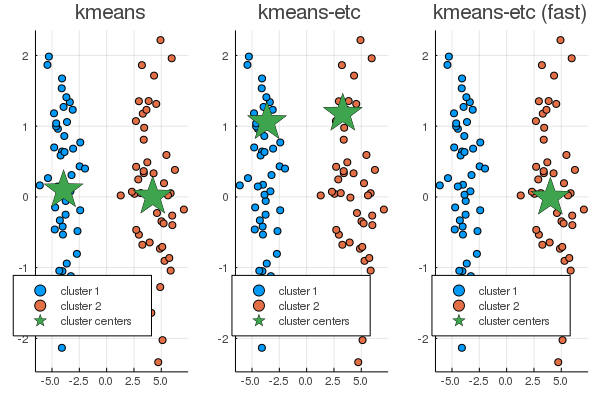
\includegraphics[width=0.5\textwidth]{figures/convex.png}
    \caption{Two unit variance Gaussian clusters with mean -4 and 4.}
\end{figure}

\begin{figure}[H]
	\centering    
    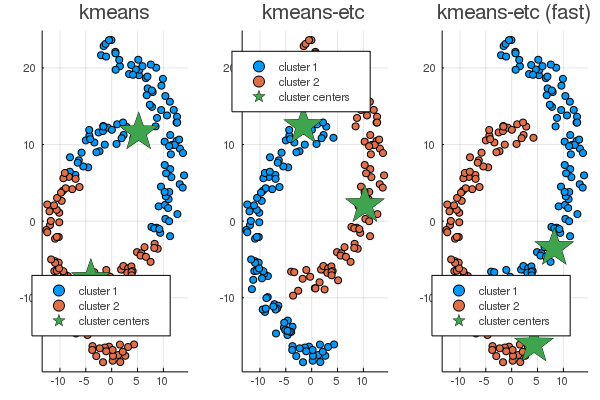
\includegraphics[width=0.5\textwidth]{figures/nonconvex.png}
    \caption{Two non-convex clusters.}
\end{figure}

Below compares scalability of the k-means, k-means using closed form pseudoinverse of ECT distance (kmeans-etc), and k-means using the iterative algorithm to estimate ECT distance (kmeans-etc (fast)). One should not take it too seriously because I did not try very hard to optimize this code. 

\begin{figure}[H]
  \begin{subfigure}[b]{0.45\textwidth}
    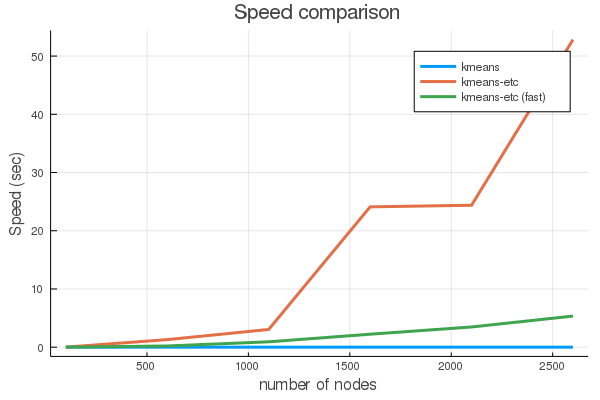
\includegraphics[width=\textwidth]{figures/speed.png}
  \end{subfigure}
  \begin{subfigure}[b]{0.45\textwidth}
    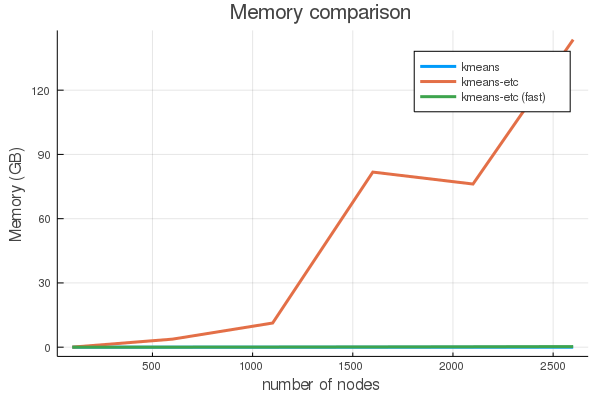
\includegraphics[width=\textwidth]{figures/memory.png}
  \end{subfigure}
\end{figure}

\section{Problems}

In honor of Ken Lange, you are required to do 2 problems. If you do more I will grade your top 2 problems. Every problem is worth the same number of points. If a problem has subproblems, each subproblem is worth the same number of points.

\begin{problembox}{Bounds of binomial coefficients}{}
For integers $n$ and $k$, prove the following inequalities
\begin{align*}
	\frac{n^k}{k^k} \le {n \choose k} \le \frac{n^k}{k!} < \left( \frac{ne}{k}\right)^k
\end{align*}
which is used in part 2 of our sharp threshold proof. For the strict inequality, rewrite $\frac{n^k}{k!} = \left(\frac{n}{k}\right)^k \frac{k^k}{k!}$ and use Taylor expansion on $e^k$.
\end{problembox}

\begin{problembox}{Verify this unproved claim}{}
Prove that $\bL^+$ in theorem 3.1 can be computed via
\begin{align*}
	\bL^+ = \left(\bL - \frac{ \bone\bone^t }{n}\right)^{-1} + \frac{\bone\bone^t}{n}
\end{align*}
where $\bone$ is a vector of 1s. This is equation (3) in \cite{fouss2007random}, but it came without a proof.
\end{problembox}

\begin{problembox}{Mandatory computational problem}{}
Starting with my code, do one of the computational problems below: 
\begin{itemize}
	\item Compute the pseudoinverse $\bL^+$ via Cholesky factorization. Recall Cholesky for $\bA\bx = \bb$ is solved via back substitution: $\bA\bx = \bb \iff \bL\bL^t\bx = \bb \iff \bL^t\bx = \by$ and $\bL\by = \bb$. Solving for $\by$ is easy because $\bL$ is lower triangular. 
	\item Recall that my code adds edges between nodes $i$ and $i+1$ as an adhoc tatic for making the graph connected. For a better alternative, \cite{yen2005clustering} suggests to add edges from a \textbf{minimal spanning tree}. In my code for computing the adjacency matrix $\bA$, compute the edges from a minimal spanning tree using your favoriate algorithm. Hopefully this solves most of our stability problem. 
\end{itemize}
\end{problembox}

\begin{problembox}{Colorings of graphs}{}
Let $K_z$ be a \textbf{complete graph} where all $z \in \Z_+$ nodes forms an edge with every other node. With equal probability, each edge is colored with red or green. Prove that $z=6$ is the minimal number of nodes needed to guarantee the existance of a \textbf{monochromatic triangle} (i.e. triangle with all edges the same color). This type of problem is what Ramsey theory studies, which we almost did. 
\end{problembox}
We have just shown $R(3, 3) = 6$. Similarly, $R(3, 4)$ is the minimal number of nodes to guarantee a red triangle or complete green rectangle (i.e. green $K_4)$. Function $R$ obviously generalizes to more colors and shapes. Using Erdos' probabilistic method, Ramsey's theorem (see \cite{sebv} or theorem 3.3 of \cite{van2001course}) says this number is finite but exponential.  This takes us to Erdos' famous quote:

\begin{displayquote}
Suppose aliens invade earth and threaten to obliterate us within a year unless human beings can find $R(5, 5)$. We could marshal the world's best minds and fastest computers, and within a year we could probably calculate the value. However, if the aliens demanded $R(6, 6)$, we would have no choice but to launch a preemptive attack.
\end{displayquote}
If you want to be famous, find $R(5, 5)$. 
\bibliographystyle{apalike}
\bibliography{references}

\end{document}